% Created 2021-01-02 Sat 17:45
% Intended LaTeX compiler: pdflatex
\documentclass[11pt]{article}
\usepackage[utf8]{inputenc}
\usepackage[T1]{fontenc}
\usepackage{graphicx}
\usepackage{grffile}
\usepackage{longtable}
\usepackage{wrapfig}
\usepackage{rotating}
\usepackage[normalem]{ulem}
\usepackage{amsmath}
\usepackage{textcomp}
\usepackage{amssymb}
\usepackage{capt-of}
\usepackage{hyperref}
\author{Me}
\date{\today}
\title{My Blog Test}
\hypersetup{
 pdfauthor={Me},
 pdftitle={My Blog Test},
 pdfkeywords={},
 pdfsubject={},
 pdfcreator={Emacs 27.1 (Org mode 9.3)}, 
 pdflang={English}}
\begin{document}

\maketitle
\tableofcontents


\section{From Graph To Score}
\label{sec:org1695886}

\subsubsection{Vectors as notes}
\label{sec:org8f8ad16}
\begin{equation}                       
\vec{a}(1 2 3 ...)                             
\end{equation} 

\begin{verbatim}
1  ;;This function will say hello
2  (defun Hello ()
3         (print "Hello World!"))
\end{verbatim}

Using "Scale" to provide a musical context for both parameters 

look at the picture 
\begin{center}
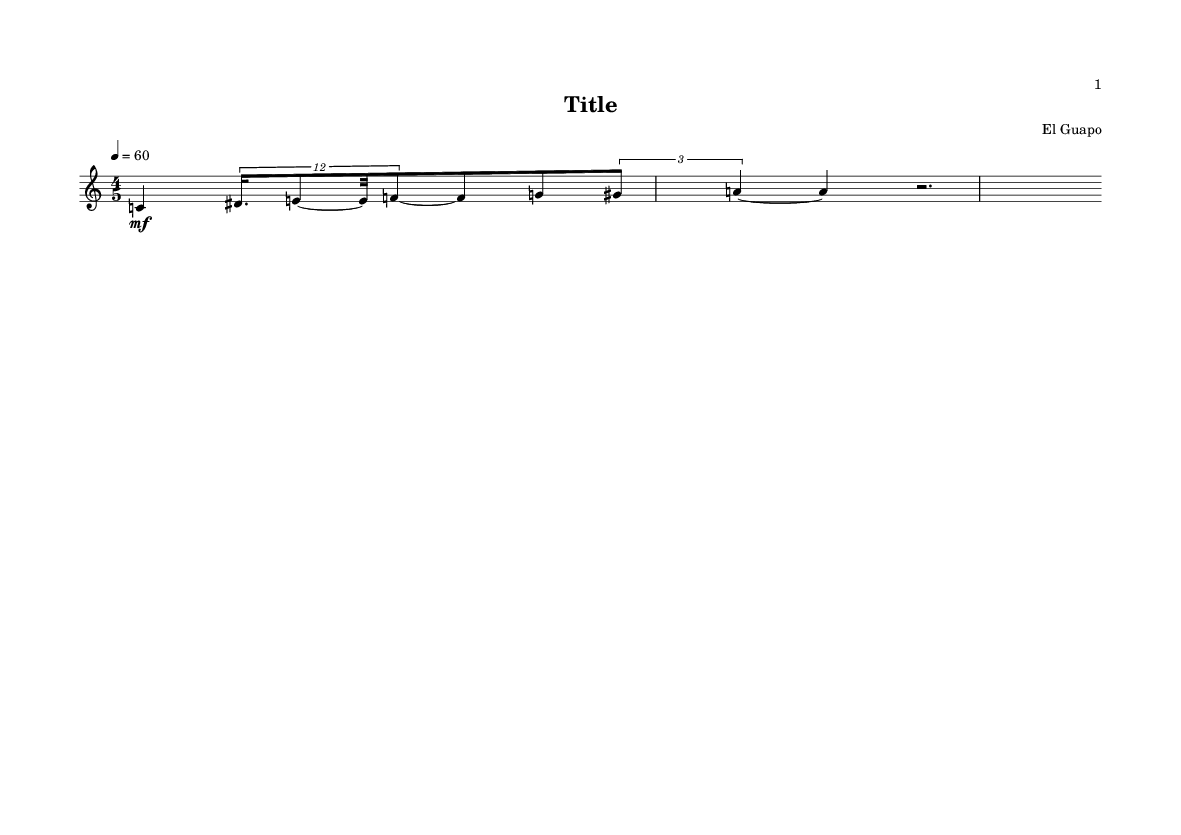
\includegraphics[width=.9\linewidth]{test.png}
\end{center}

Oh! check out this SVG:
\begin{center}
\includesvg[width=.9\linewidth]{graphtest}
\end{center}
\end{document}